\section{System architecture}
\label{sec:sys_arch}

The developed 4D GIS has a two-tier {\em client-server} architecture. The {\em server} contains the master copy of all the involved data and a PostgreSQL database called \textit{viaappiadb} to ease the data handling. Both are used for data preparation, i.e. converting the data to the required formats for the available viewers. These run in the laptops of the archaeological researchers ({\em clients}) where local copies of the converted data in the {\em server} are downloaded when required.

\subsection{Data preparation at server}

A diagram of the data preparation procedure which is carried out in the {\em server} is shown in Figure \ref{fig:sys_arch_data_framework}. As explained in section \ref{sec:concept_descr}) for the whole area, conceptually referred as background, we have only point cloud data, while for the individual monuments, conceptually referred as sites, the data is of more types (point clouds, meshes, pictures, 2D footprints and attributes). 

In order to run the Windows desktop viewer in the clients the raw data has to be converted to the OpenSceneGraph
(\url{http://www.openscenegraph.org}) binary format. The web-based viewer is using the POTree (\url{http://potree.org/}) WebGL point
cloud visualization framework and the data needs to be converted with the POTree Converter which restructures the data into a OctTree where each leaf node is a file of format LAS or LAZ. 

During the data preparation process the \textit{viaappiadb} database is filled with
meta-data information which contains the raw data location and converted data location.
Furthermore, the archaeological information with attribute data for the several sites
is extracted from a Microsoft Access file and imported into the \textit{viaappiadb}. The footprints are provided in a ShapeFile and they are also imported into the \textit{viaappiadb} database as well. In addition, altitude
ranges for the sites are derived from the PC raw data in combination with the footprints and they are also added
to the database. On Figures \ref{fig:sys_arch_data_framework} and \ref{fig:sys_arch_2tier}
the solid arrows indicate data flow, while the dashed arrows indicate meta-data flow
during the data preparation process.

\begin{figure}[H] \centering
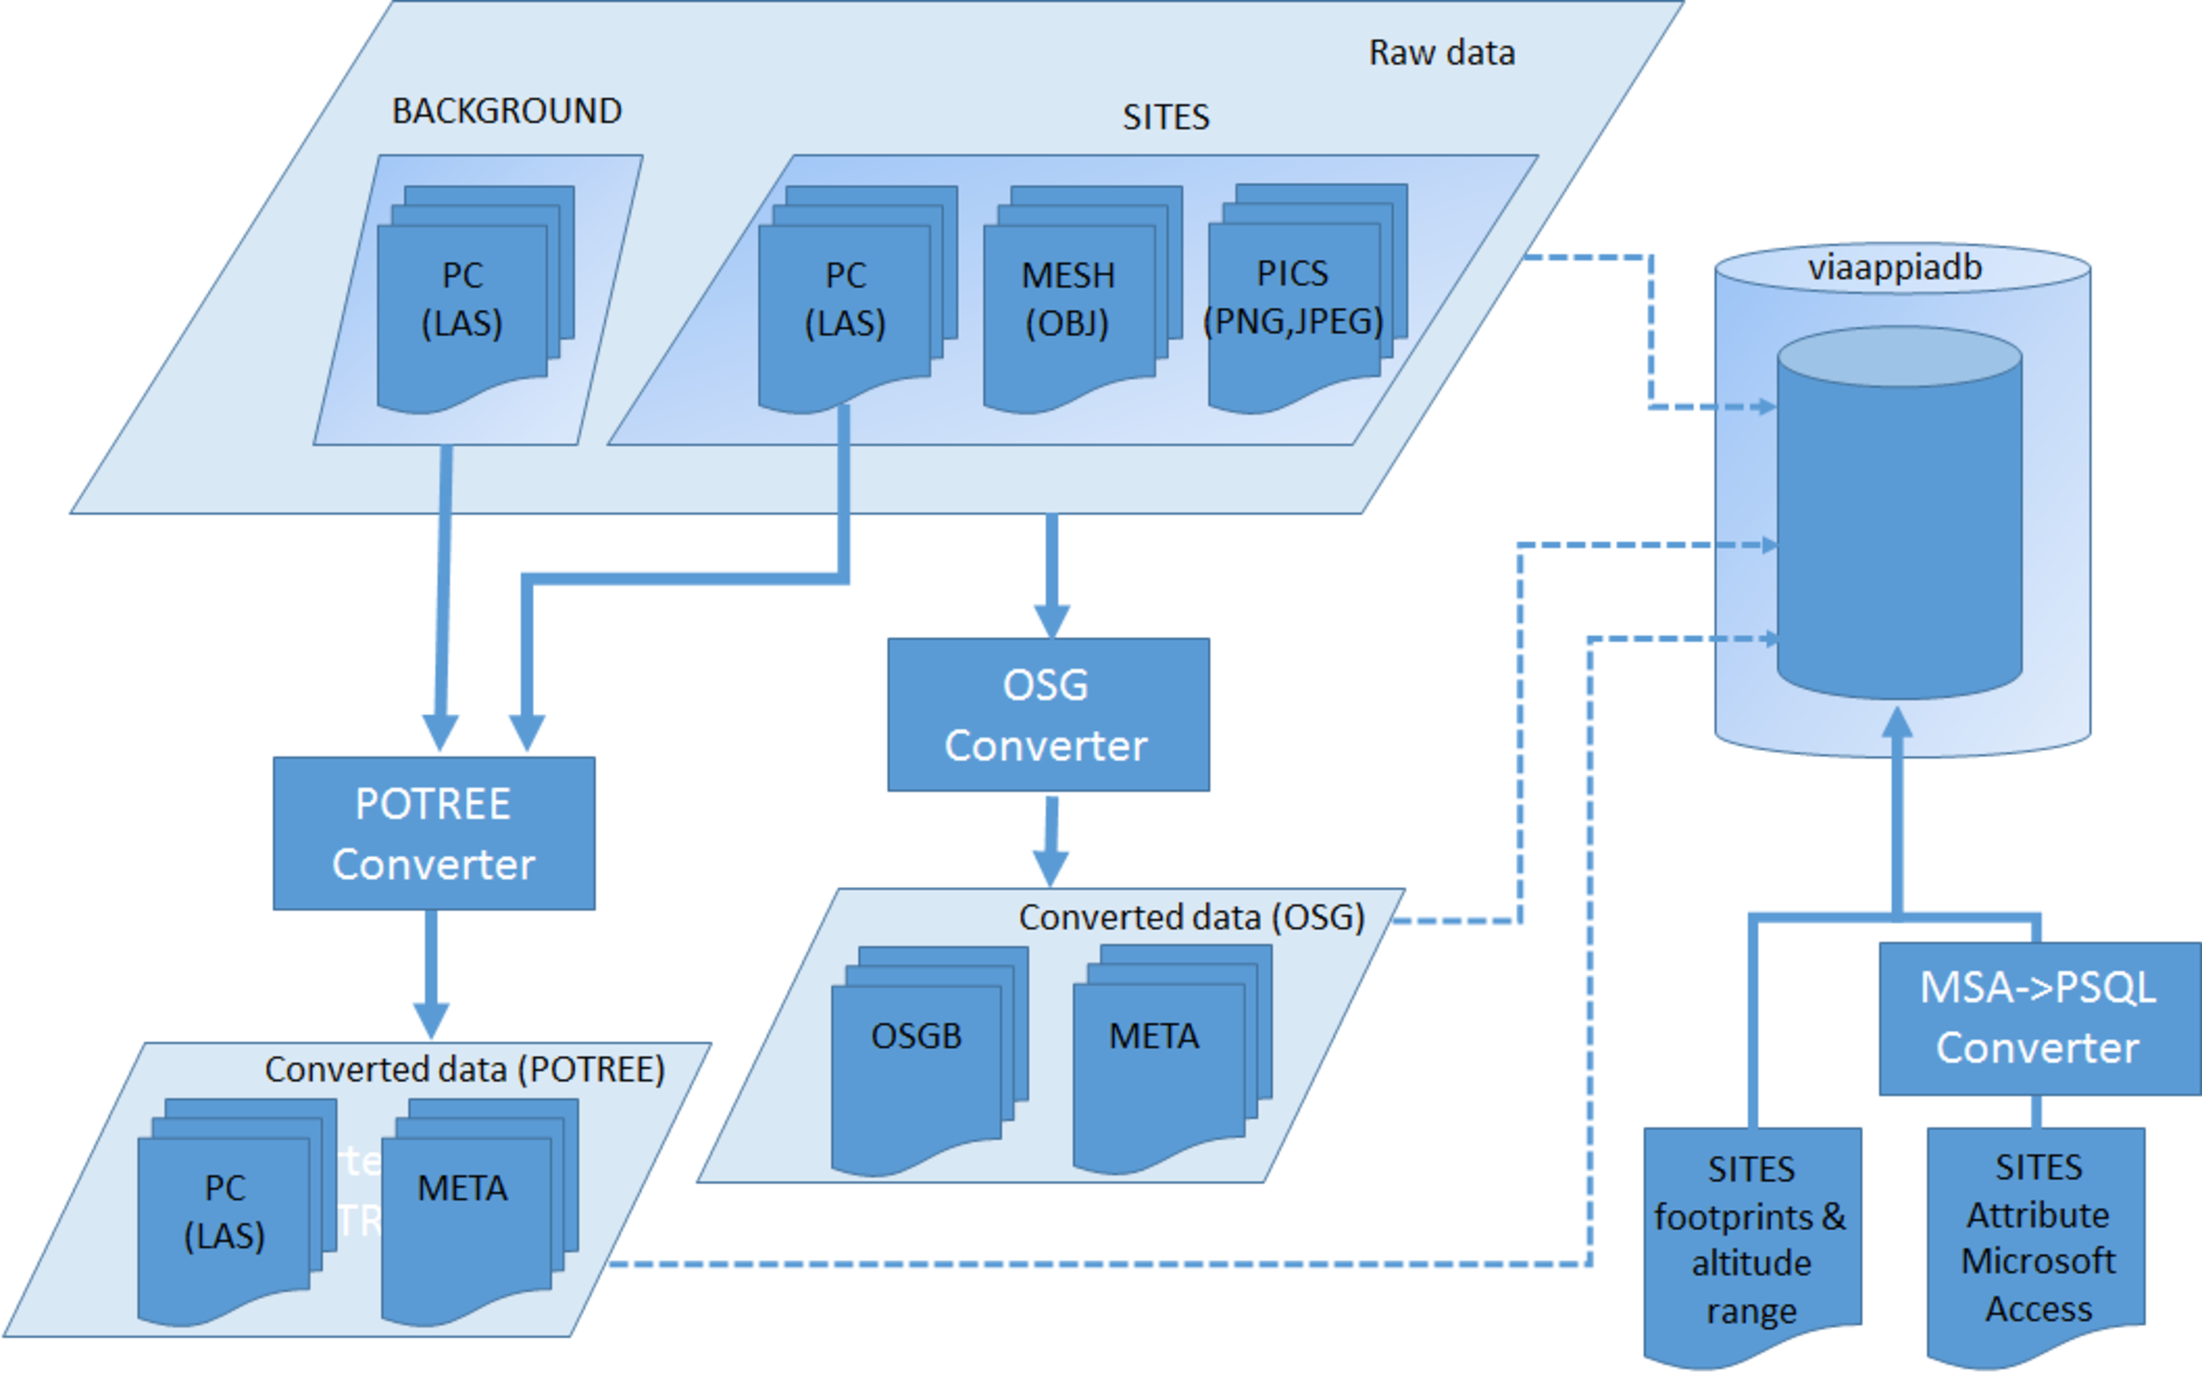
\includegraphics[width=0.75\textwidth]{fig/system_architecture/DataFramework.pdf}
\caption{Data preparation framework executed on the Via Appia Linux serer}
\label{fig:sys_arch_data_framework} \end{figure}

\subsection{Visualization at clients}

Once the data preparation framework has concluded its task the data is made available
for multi-client sessions. In the case of Windows desktop viewers a local copy of all the OSG data is required before initializing the viewer.

A \textit{launcher} tool based on the Xenon library (\url{http://nlesc.github.io/Xenon/}),
developed by the Netherlands eScience Center (NLeSC), makes sure the local copy is
synchronized with the server. It also retrieves from the server the configuration
file required by the desktop viewer. Once the synchronization finishes the launcher
is in charge of starting the viewer. In the end of a session the launcher updates
the remote database using the modified configuration file. Offline operational
mode is also provided, this is, the user decides when to synchronize and takes care of it.

For the Web-based viewer it is not required a local copy of the entire Potree converted
data. The necessary data is pulled automatically by the web application from the server on request via a NGINX Web server
(\url{nginx.com}). Such data also includes a JSON configuration file containing the
meta-data for the background and sites information extracted from the {\em viaappia}
database. The 3D Web-based viewer have been developed by NLeSC. Figure \ref{fig:sys_arch_2tier}
illustrates the two-tier architecture and shows the steps performed at the client
side. 

All the process described so far has been automated. Section~\ref{sec:software} contains
more detailed information about the architecture. 


\begin{figure}[H] \centering
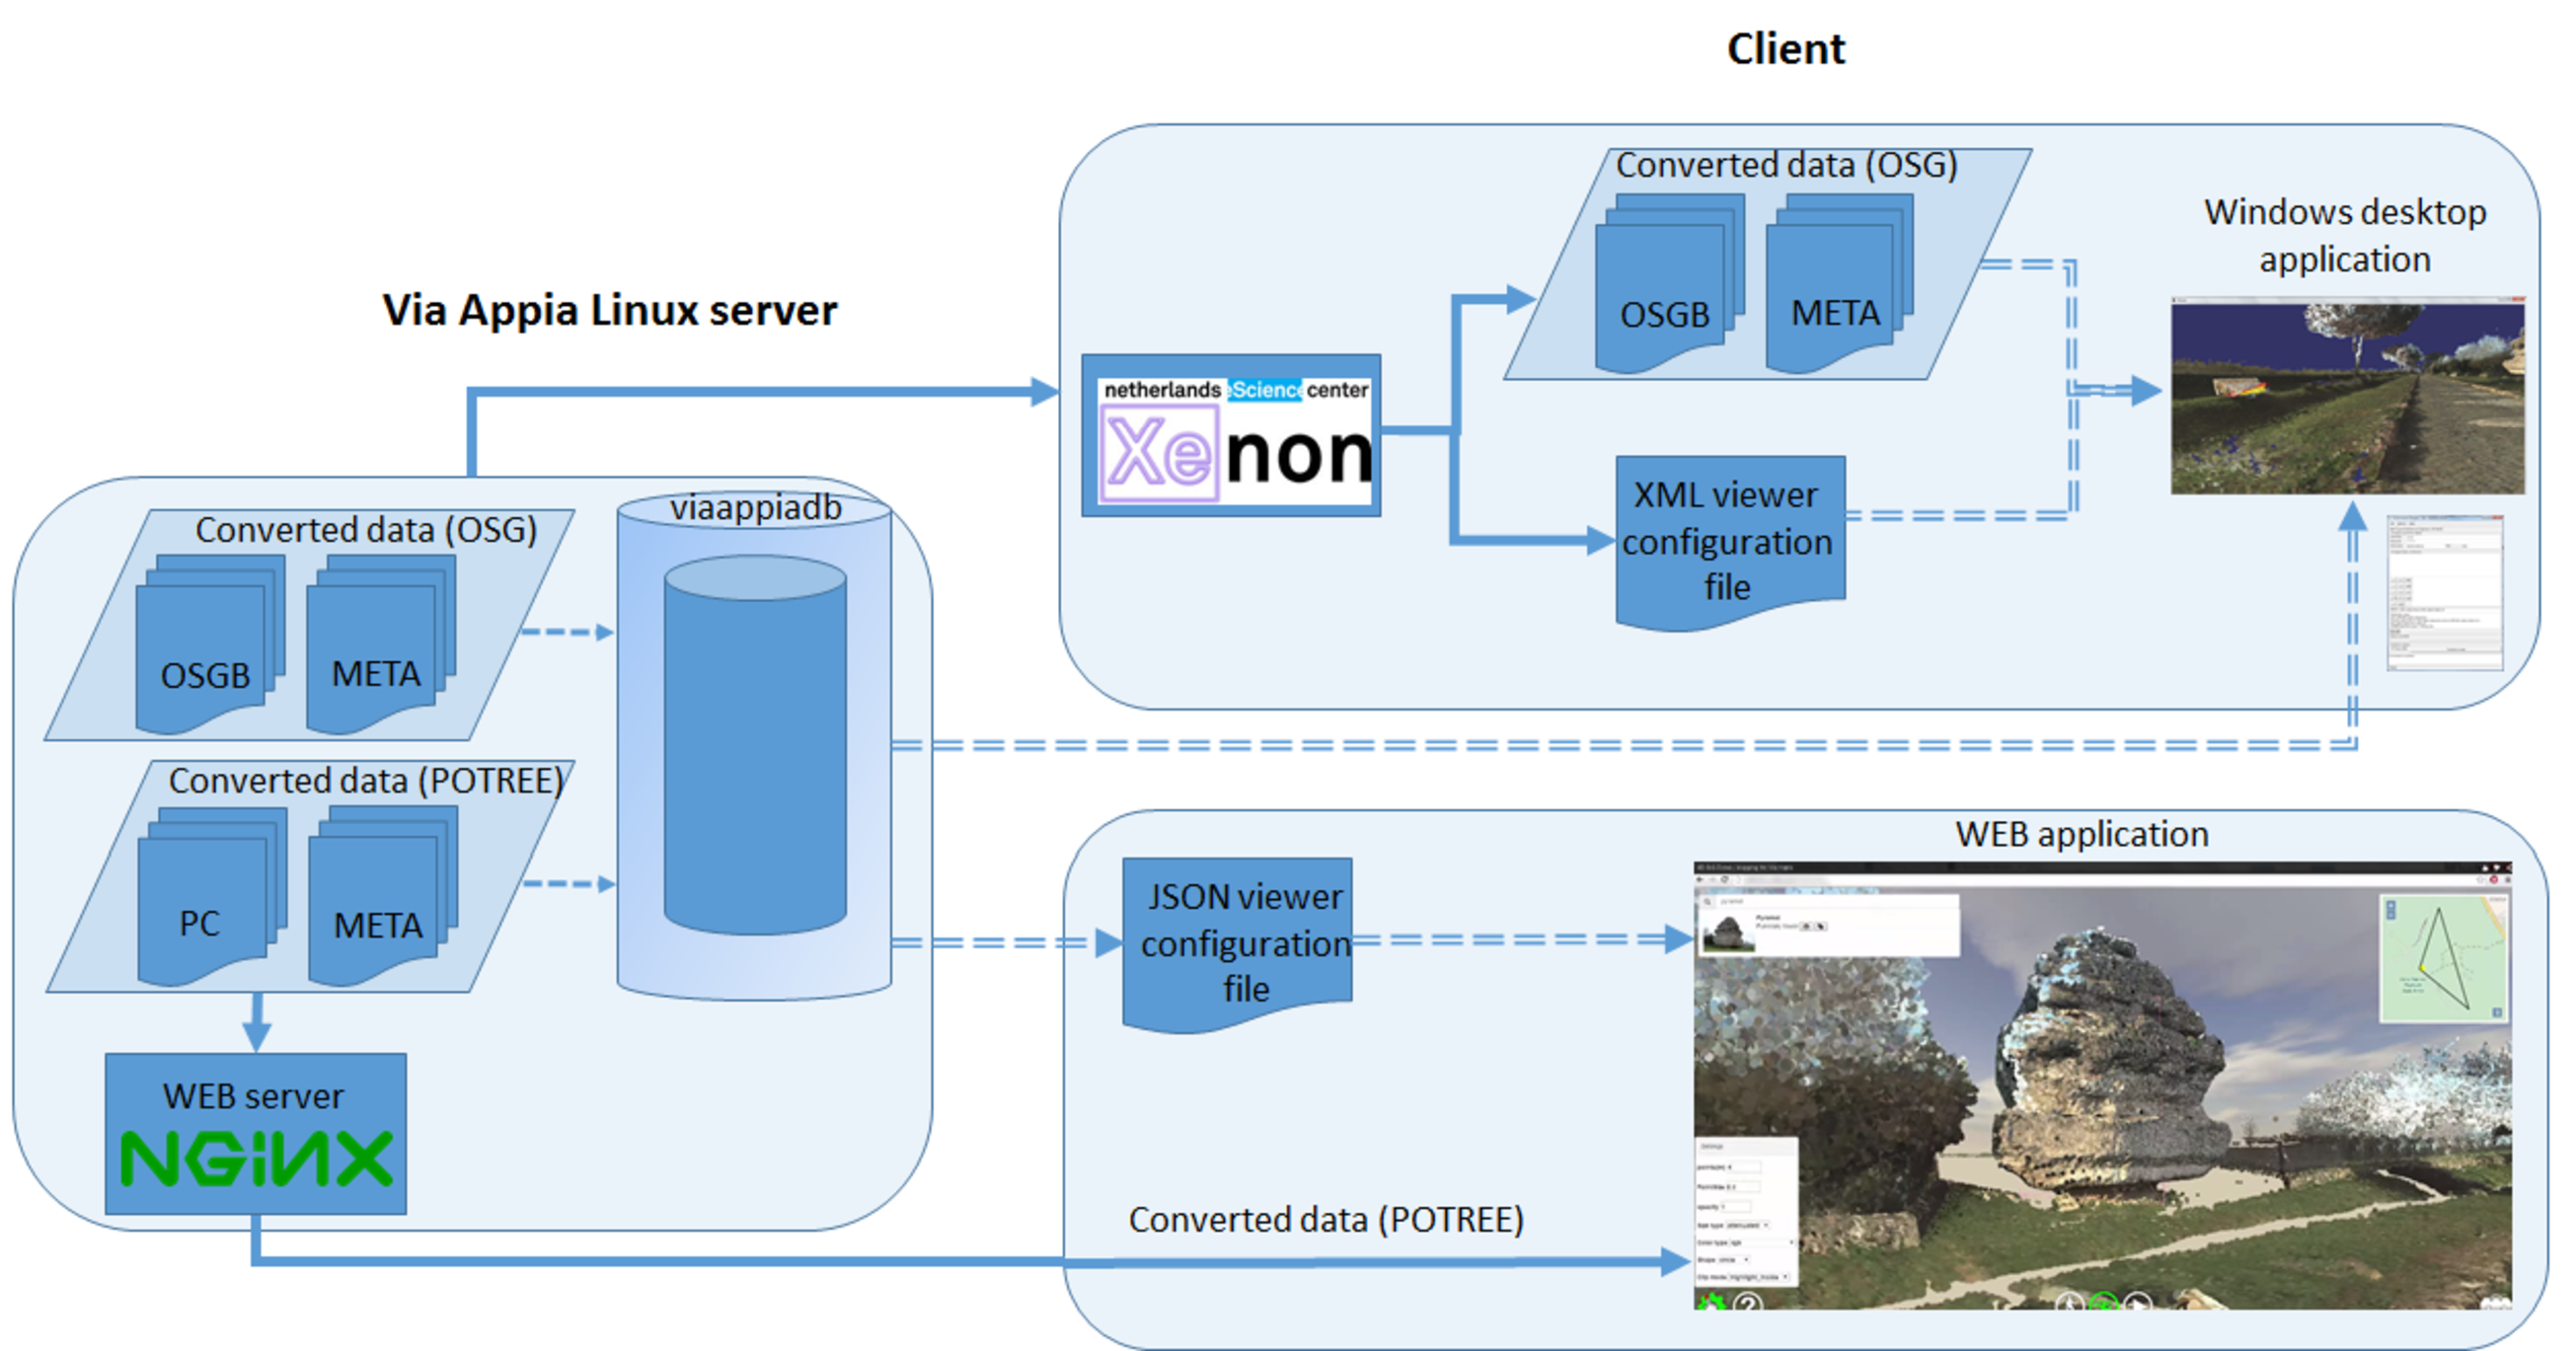
\includegraphics[width=0.95\textwidth]{fig/system_architecture/TwoTierArchitecture.pdf}
\caption{Two-tier architecture of the Via Appia 4D GIS and the steps
executed on the client side.} \label{fig:sys_arch_2tier} \end{figure}
